% This example is meant to be compiled with lualatex or xelatex
% The theme itself also supports pdflatex
\PassOptionsToPackage{unicode}{hyperref}
\documentclass[aspectratio=1610, 12pt]{beamer}

% Warning, if another latex run is needed
% \usepackage[aux]{rerunfilecheck}

% just list chapters and sections in the toc, not subsections or smaller
\setcounter{tocdepth}{1}

%------------------------------------------------------------------------------
%------------------------------ Fonts, Unicode, Language ----------------------
%------------------------------------------------------------------------------
\usepackage{fontspec}
\defaultfontfeatures{Ligatures=TeX}  % -- becomes en-dash etc.

% german language
\usepackage{polyglossia}
\setdefaultlanguage{german}

% for english abstract and english titles in the toc
\setotherlanguages{english}

% intelligent quotation marks, language and nesting sensitive
\usepackage[autostyle]{csquotes}

% microtypographical features, makes the text look nicer on the small scale
\usepackage{microtype}

%------------------------------------------------------------------------------
%------------------------ Math Packages and settings --------------------------
%------------------------------------------------------------------------------

\usepackage{amsmath}
\usepackage{amssymb}
\usepackage{mathtools}
\usepackage{bbold}

% Enable Unicode-Math and follow the ISO-Standards for typesetting math
\usepackage[
  math-style=ISO,
  bold-style=ISO,
  sans-style=italic,
  nabla=upright,
  partial=upright,
]{unicode-math}
\setmathfont{Latin Modern Math}

% nice, small fracs for the text with \sfrac{}{}
\usepackage{xfrac}


%------------------------------------------------------------------------------
%---------------------------- Numbers and Units -------------------------------
%------------------------------------------------------------------------------

\usepackage[
  locale=DE,
  separate-uncertainty=true,
  per-mode=symbol-or-fraction,
]{siunitx}
\sisetup{math-micro=\text{µ},text-micro=µ}
% \sisetup{tophrase={{ to }}}
%------------------------------------------------------------------------------
%-------------------------------- tables  -------------------------------------
%------------------------------------------------------------------------------

\usepackage{booktabs}       % \toprule, \midrule, \bottomrule, etc

%------------------------------------------------------------------------------
%-------------------------------- graphics -------------------------------------
%------------------------------------------------------------------------------

\usepackage{graphicx}
%\usepackage{rotating}
\usepackage{grffile}
\usepackage{tikz}
\usepackage{circuitikz}
\usepackage{tikz-feynman}
\usepackage{subcaption}

% allow figures to be placed in the running text by default:
\usepackage{scrhack}
\usepackage{float}
\floatplacement{figure}{htbp}
\floatplacement{table}{htbp}

% keep figures and tables in the section
\usepackage[section, below]{placeins}

% smileys
\usepackage{MnSymbol,wasysym}

%------------------------------------------------------------------------------
%---------------------- customize list environments ---------------------------
%------------------------------------------------------------------------------

\usepackage{enumitem}
\usepackage{listings}
\usepackage{hepunits}

\usepackage{pdfpages}
%------------------------------------------------------------------------------
%------------------------------ Bibliographie ---------------------------------
%------------------------------------------------------------------------------

\usepackage[
  backend=biber,   % use modern biber backend
  autolang=hyphen, % load hyphenation rules for if language of bibentry is not
                   % german, has to be loaded with \setotherlanguages
                   % in the references.bib use langid={en} for english sources
]{biblatex}
\addbibresource{references.bib}  % the bib file to use
\DefineBibliographyStrings{german}{andothers = {{et\,al\adddot}}}  % replace u.a. with et al.


% Load packages you need here
% \usepackage{polyglossia}
% \setmainlanguage{german}

\usepackage{csquotes}


% \usepackage{amsmath}
% \usepackage{amssymb}
% \usepackage{mathtools}

\usepackage{hyperref}
\usepackage{bookmark}

% load the theme after all packages

\usetheme[
  showtotalframes, % show total number of frames in the footline
]{tudo}

% Put settings here, like
\unimathsetup{
  math-style=ISO,
  bold-style=ISO,
  nabla=upright,
  partial=upright,
  mathrm=sym,
}

% \setbeamertemplate{itemize item}{\scriptsize$\blacktriangleright$}
% \setbeamertemplate{itemize subitem}{\scriptsize$\blacktriangleright$}

%Titel:
\title{Stability measurement for SciFi module alignment on 2022 data}
%\subtitle{tuning of uncertainties}
%Autor
\author[N.Breer]{Nils Breer}
%Lehrstuhl/Fakultät
\institute{TU Dortmund, AG Albrecht}
%\titlegraphic{\includegraphics[width=0.3\textwidth]{content/Bilder/interferenz.jpg}}
% \date{12.05.2023}

\begin{document}
\maketitle

\begin{frame}\frametitle{Motivation and procedure}
  \begin{columns}
    \begin{column}[c]{0.4\textwidth}
      \begin{itemize}
        \setlength\itemsep{1em}
        \item $\bullet$\, \textbf{How much does the SciFi move between runs?}
        \item $\bullet$\, \textbf{Does magUp vs. magDown polarity impact the movement?}
      \end{itemize}
    \end{column}
    \begin{column}[c]{0.6\textwidth}
      \begin{itemize}
        \item $\bullet$\, Run an alignment for each of the runs on the list
        \item $\bullet$\, Sort the runs in ascending run number
        \item $\bullet$\, Compare the difference in module position for each run to the next
        \item $\bullet$\, Where are the modules in the local frame in all runs?
      \end{itemize}
    \end{column}
  \end{columns}
\end{frame}

\begin{frame}\frametitle{Dataset and Alignment setup}
  \begin{columns}
    \begin{column}[c]{0.9\textwidth}
      \begin{itemize}
        \setlength\itemsep{0em}
        \item $\bullet$\, \href{https://twiki.cern.ch/twiki/bin/viewauth/LHCbInternal/CommissioningData2022}{Dataset} contains magUp and magDown samples from 2022 labeled as "good" from EMTF
        \item $\bullet$\, Good: > 90\% of datalinks are good
        \item $\bullet$\, Includes runs from fills: 8489, 8491, 8496
        \item List of randomly chosen runs: 255949, 256030, 256145, 256159, 256163, 256272, 256278, 256290
        \item $\bullet$\, V10 \href{https://indico.cern.ch/event/1283973/contributions/5394548/attachments/2642212/4572628/Alignv3_summary.pdf}{Alignment} from tag (loose tracking, half module alignment TxTz + Mats, back layer fixed) from conditions database
      \end{itemize}
    \end{column}
  \end{columns}
\end{frame}

\begin{frame}\frametitle{Module Positions in local half module frame}
  \begin{columns}
    \begin{column}[c]{0.35\textwidth}
      \begin{itemize}
        \setlength\itemsep{0em}
        \item $\bullet$\, Runs 255949 + 256030 were from fill 8489
        \item $\bullet$\, Optimal fine timing implemented in 256145 (afterwards)
        \item $\bullet$\, Positions of other runs compatible
        \item $\bullet$\, magUp: 256272, 256278, 256290
        \item $\bullet$\, magDown: 255949, 256030, 256145, 256159, 256163
      \end{itemize}
    \end{column}
    \begin{column}[c]{0.65\textwidth}
      \begin{figure}
        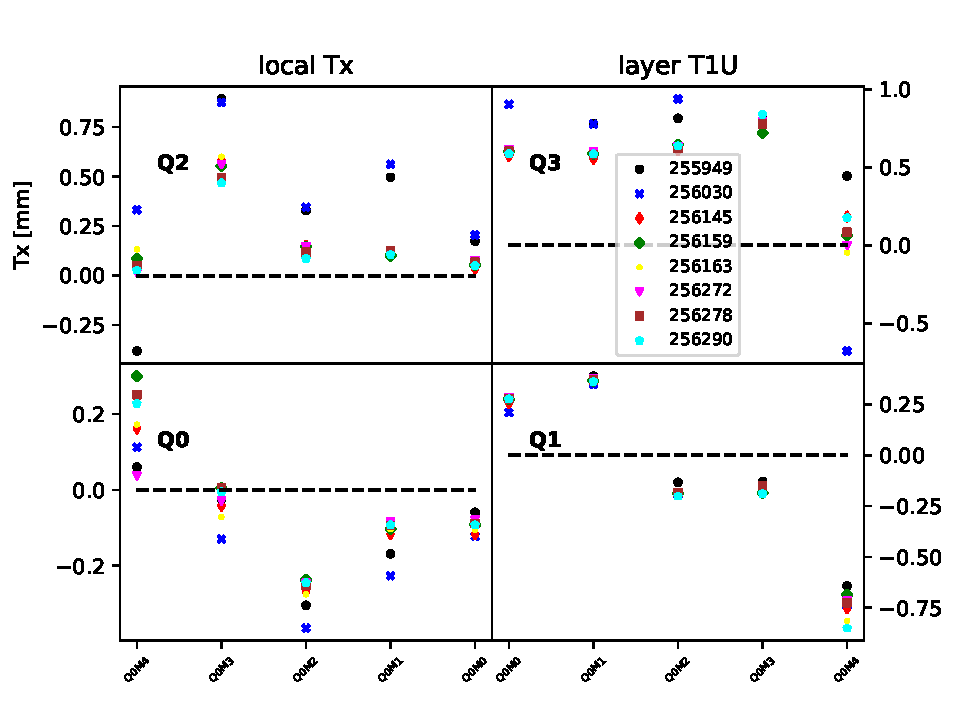
\includegraphics[width=0.9\textwidth]{plots/plain_data/raw_data_T1U_Tx.pdf}
      \end{figure}
    \end{column}
  \end{columns}
\end{frame}

\begin{frame}\frametitle{Module positions: magUp and magDown in x-direction}
  \begin{itemize}
    \setlength\itemsep{0em}
    \item $\bullet$\, magUp (left) and magDown (right) runs are compatible respectively within $100 \mu m$
    \item $\bullet$\, black, \textcolor{blue}{blue}: worse timing than other runs \to shifted modules
    % \item $\bullet$\, Introducing a different timing: shift by up to 1 $mm$ in the outer modules,
  \end{itemize}
  \begin{columns}
    \begin{column}[c]{0.48\textwidth}
      \begin{figure}
        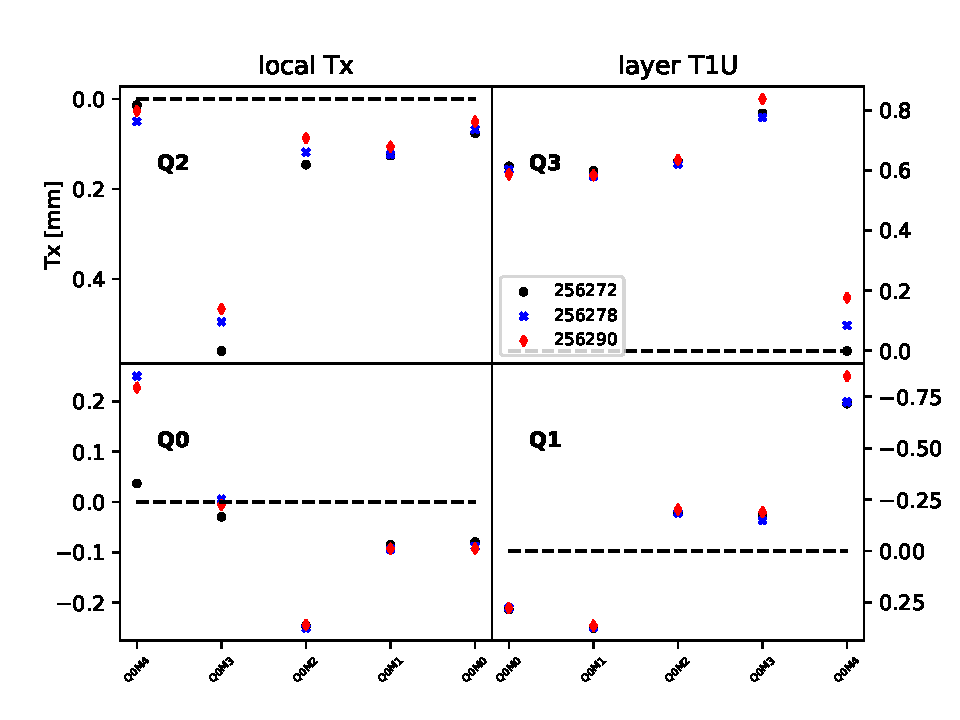
\includegraphics[width=\textwidth]{plots/plain_data/raw_MU_T1U_Tx.pdf}
      \end{figure}
    \end{column}
    \begin{column}[c]{0.48\textwidth}
      \begin{figure}
        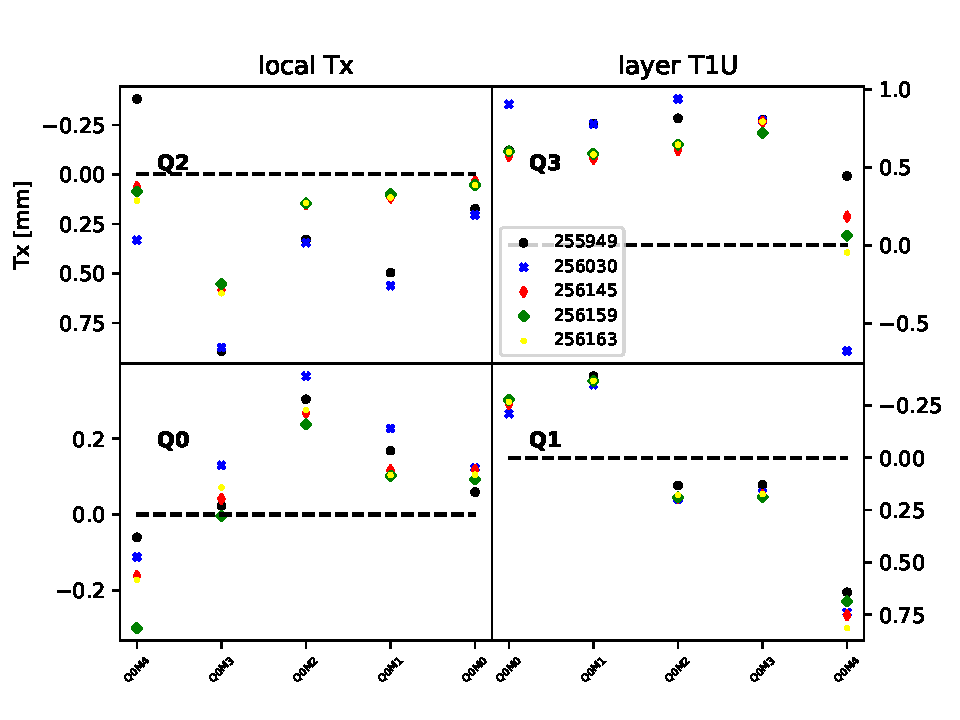
\includegraphics[width=\textwidth]{plots/plain_data/raw_MD_T1U_Tx.pdf}
      \end{figure}
    \end{column}
  \end{columns}
\end{frame}

\begin{frame}\frametitle{Difference between runs: Tx}
  \begin{columns}
    \begin{column}[c]{0.48\textwidth}
      \begin{itemize}
        \setlength\itemsep{0em}
        \item $\bullet$\, difference in module position between 2 runs
        \item $\bullet$\, Outer module (M4) more movement than inner modules (\approx 280 hits in M4 vs 100k hits in M0)
        \item $\bullet$\, 256030 to 256145 (\textcolor{blue}{blue} markers) largest movement: fine timing changes, lack of statistics
        \item $\bullet$\, Timing changes: expect movement of at most $250 \mu m$ if enough statistics
        \item $\bullet$\, largest movements/outliers (blue markers): T1VQ2M2 (-0.4$\text{mm}$), T3VQ2M{3,4} (-0.8$\text{mm}$), T3X2M{3,4} (-0.6$\text{mm}$)
        % \item \to possible cause: lack of statistics
      \end{itemize}
    \end{column}
      \begin{column}[c]{0.48\textwidth}
        \begin{figure}
          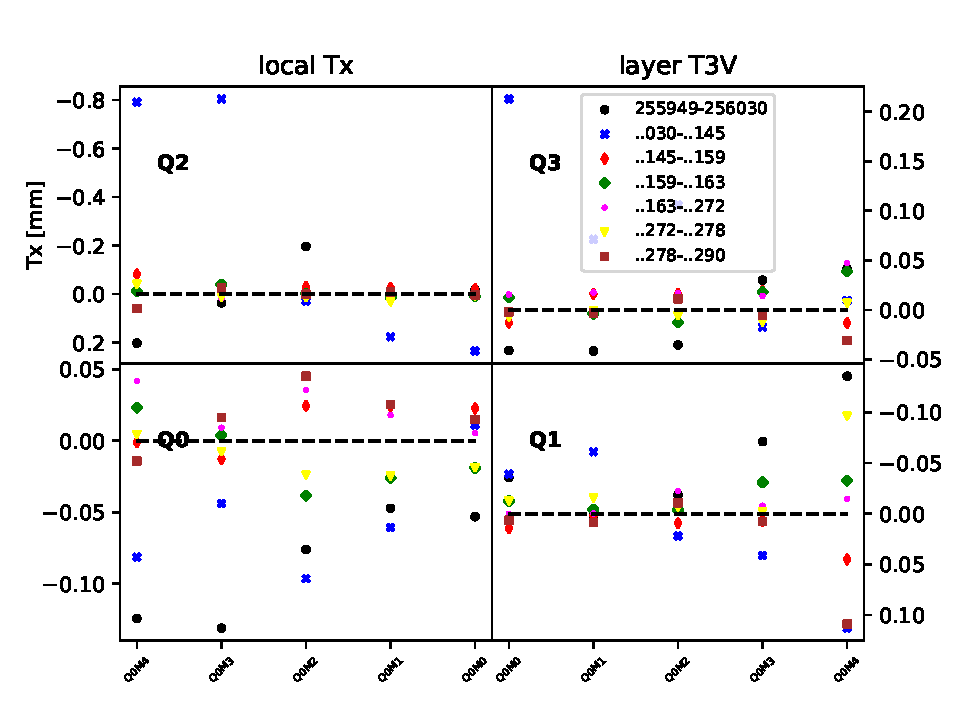
\includegraphics[width=\textwidth]{plots/stability_plots/diff_data_T3V_Tx.pdf}
        \end{figure}
      \end{column}
  \end{columns}
\end{frame}

\begin{frame}\frametitle{Reduced dataset: removed pre timing update runs}
  \begin{columns}
    \begin{column}[c]{0.48\textwidth}
      \begin{itemize}
        % \item $\bullet$\, removed the first 2 runs from input list since they are from a fill without the optimal timing changes
        \item $\bullet$\, again: compare module positions of 2 runs but remove first 2 runs from input (different fine timing)
        \item $\bullet$\, Without the fine timing changes the largest movement is at max around $400 \mu m$ at most outer modules
        \item $\bullet$\, M4, M5 often < 1000 events (difficult for the alignment) \to large movement,
        \item $\bullet$\, M0-M3: movement around $150 \mu m$
      \end{itemize}
    \end{column}
      \begin{column}[c]{0.48\textwidth}
        \begin{figure}
          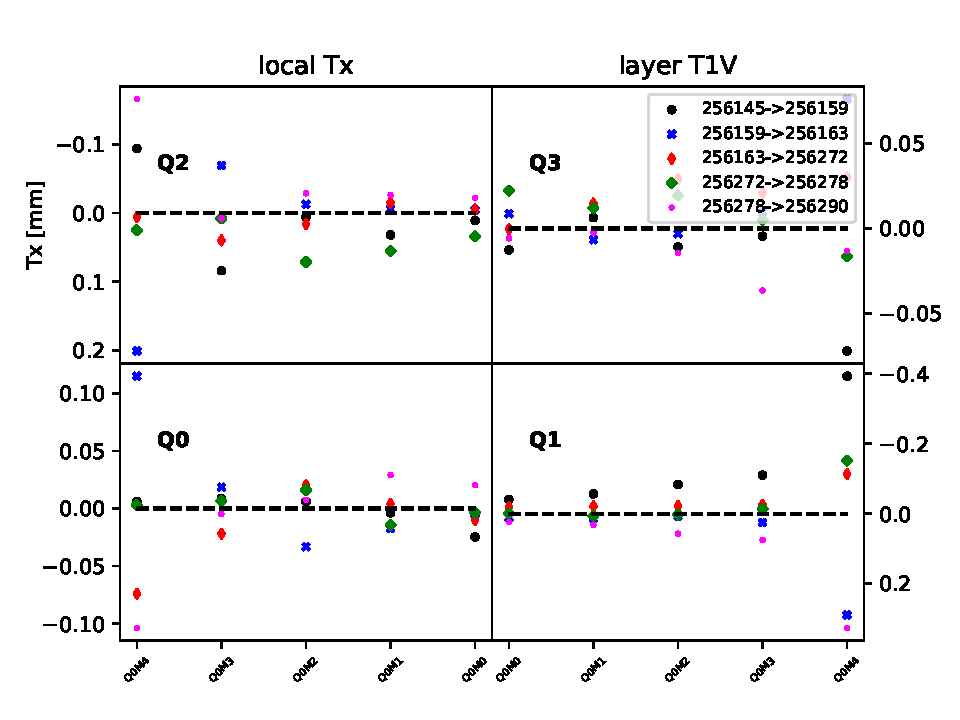
\includegraphics[width=\textwidth]{plots/stability_plots/diff_reduced_Tx_T1V_Tx.pdf}
        \end{figure}
      \end{column}
  \end{columns}
\end{frame}

% \begin{frame}\frametitle{Difference between runs: Tz}
%   \begin{columns}
%     \begin{column}[c]{0.48\textwidth}
%       \begin{itemize}
%         \item $\bullet$\, Tz a little worse in performance as expected
%         \item $\bullet$\, similar picture as for Tx
%         % \item $\bullet$\,
%       \end{itemize}
%     \end{column}
%     \begin{column}[c]{0.48\textwidth}
%       \begin{figure}
%         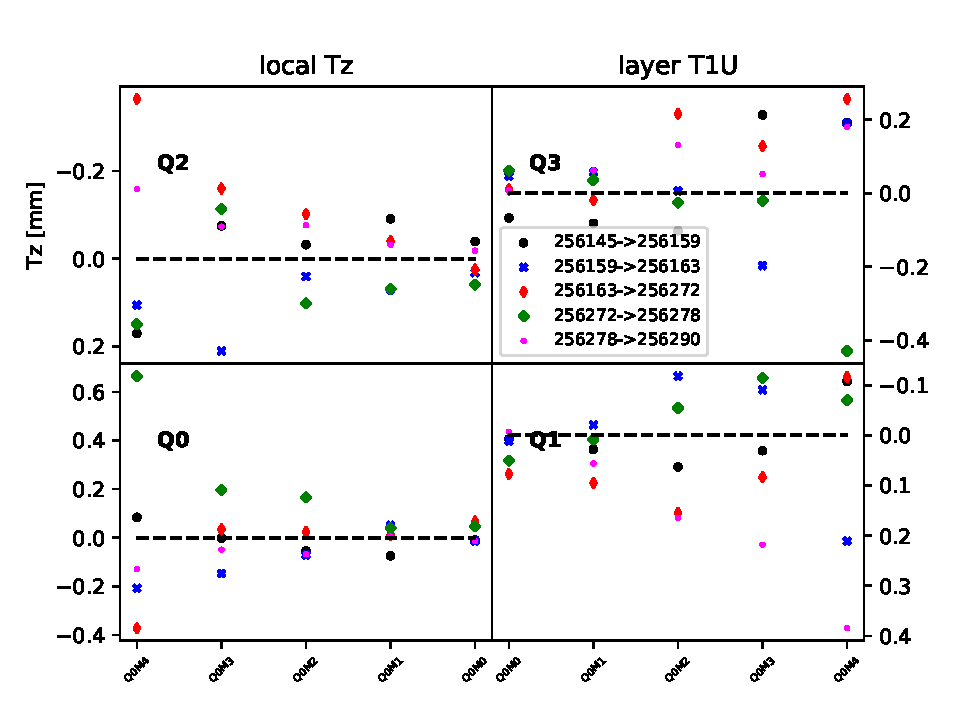
\includegraphics[width=0.7\textwidth]{plots/stability_plots/diff_reduced_Tz_T1U_Tz.pdf}
%       \end{figure}
%     \end{column}
%   \end{columns}
% \end{frame}

\begin{frame}\frametitle{Conclusion}
  \begin{columns}
    \begin{column}[c]{\textwidth}
      \begin{itemize}
        \item $\bullet$\, Impactful changes like timing induces an observed movement up to 0.8mm in some cases
        \item $\bullet$\, The change in module position from run to run is at maximum $150 \mu m$ for the modules M0 \to M3 in Tx
        \item \to only if there are no big changes between runs
        \item $\bullet$\, M4 moves at max $400 \mu m$ in this case
        \item $\bullet$\, there is no visible difference between magUp and magDown polarity
        \item $\bullet$\, With good SciFi timing, variation of 200 $\mu m$ expected.
        \item $\bullet$\, A possible choice of an automatic update would be if variations of > 200 $\mu m$ occur.
      \end{itemize}
    \end{column}
  \end{columns}
\end{frame}

\begin{frame}\frametitle{Backup: MagUp and magDown only comparison}
  MagUp Tx and Tz module position comparisons
  \begin{columns}
    \begin{column}[c]{0.48\textwidth}
      \begin{figure}
        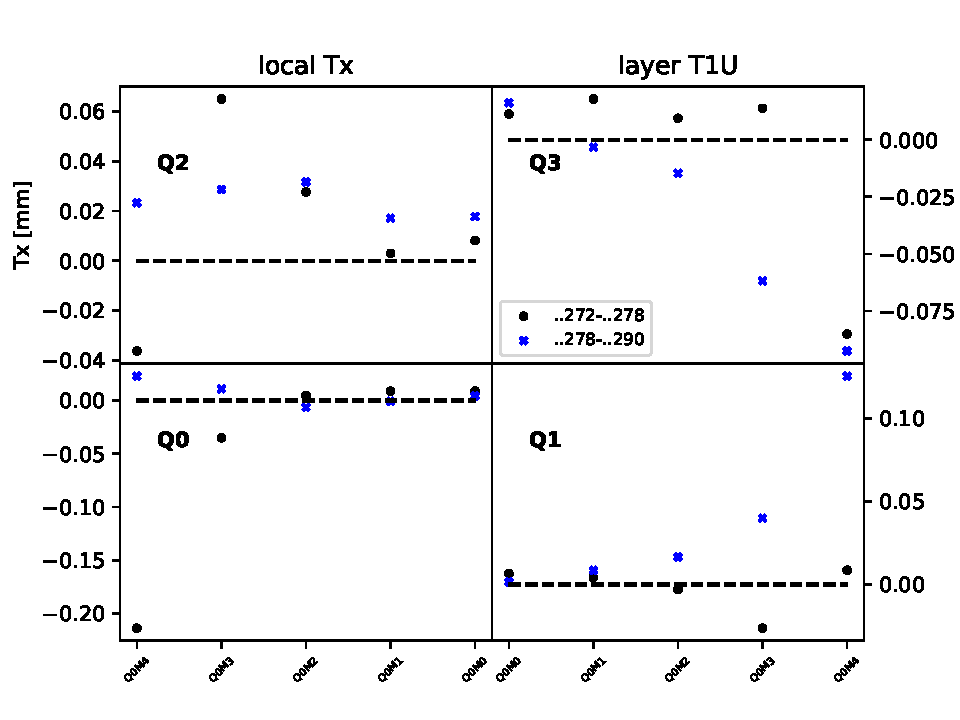
\includegraphics[width=\textwidth]{plots/stability_plots/diff_MU_T1U_Tx.pdf}
      \end{figure}
    \end{column}
    \begin{column}[c]{0.48\textwidth}
      \begin{figure}
        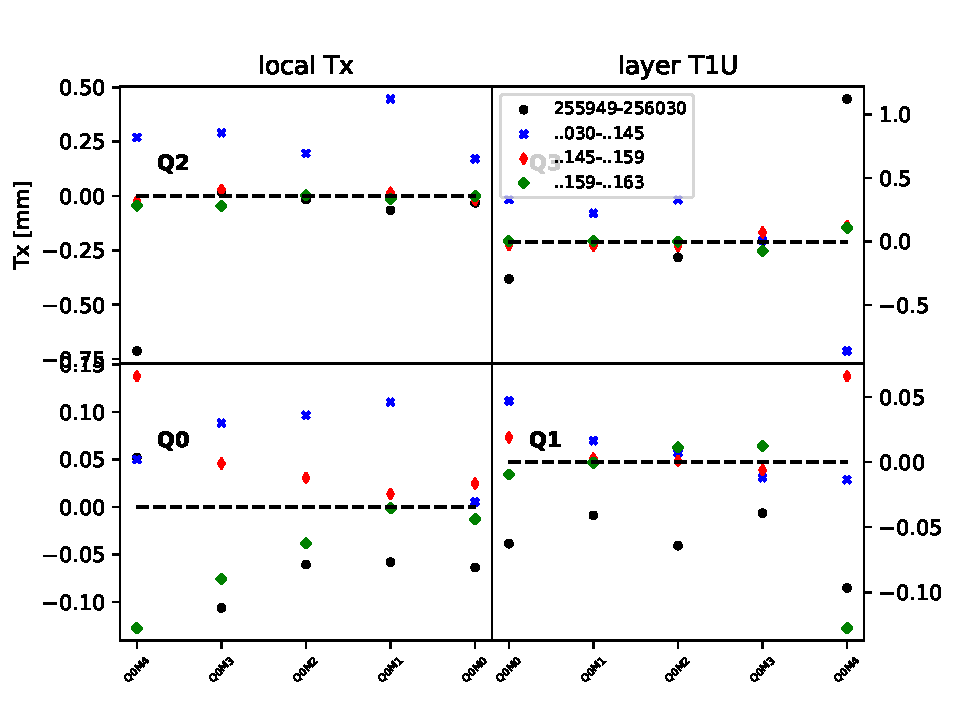
\includegraphics[width=\textwidth]{plots/stability_plots/diff_MD_T1U_Tx.pdf}
      \end{figure}
    \end{column}
    % \begin{column}[c]{0.48\textwidth}
    %   \begin{figure}
    %     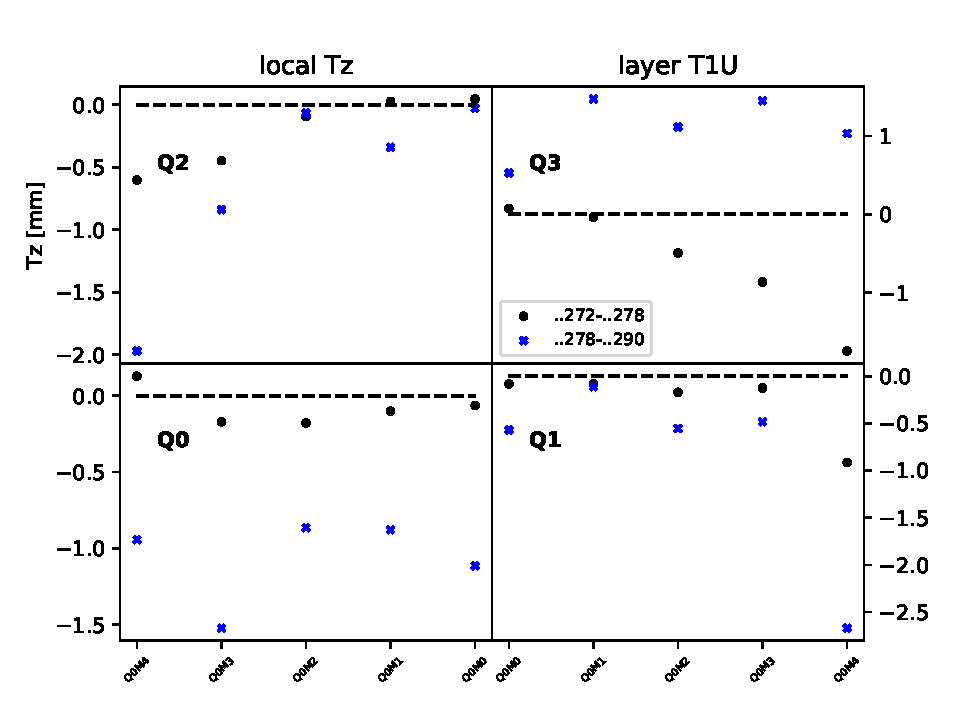
\includegraphics[width=0.9\textwidth]{plots/stability_plots/diff_MU_T1U_Tz.pdf}
    %   \end{figure}
    % \end{column}
  \end{columns}
\end{frame}

% \begin{frame}\frametitle{Backup}
%   MagDown Tx and Tz module position comparisons
%   \begin{columns}
%     \begin{column}[c]{0.48\textwidth}
%       \begin{figure}
%         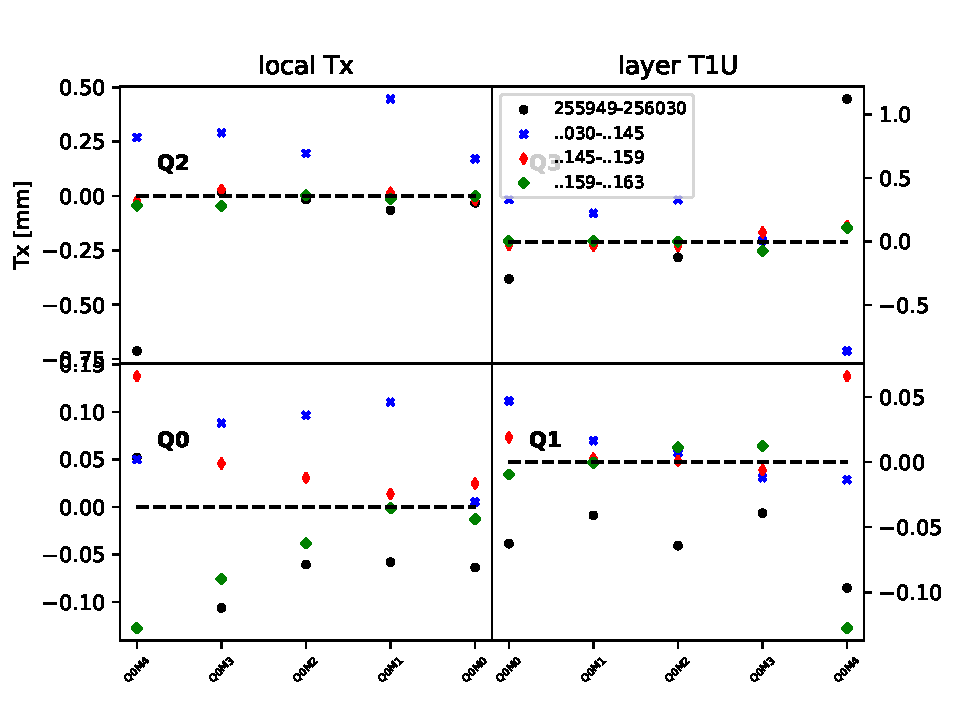
\includegraphics[width=0.9\textwidth]{plots/stability_plots/diff_MD_T1U_Tx.pdf}
%       \end{figure}
%     \end{column}
%       \begin{column}[c]{0.48\textwidth}
%         \begin{figure}
%           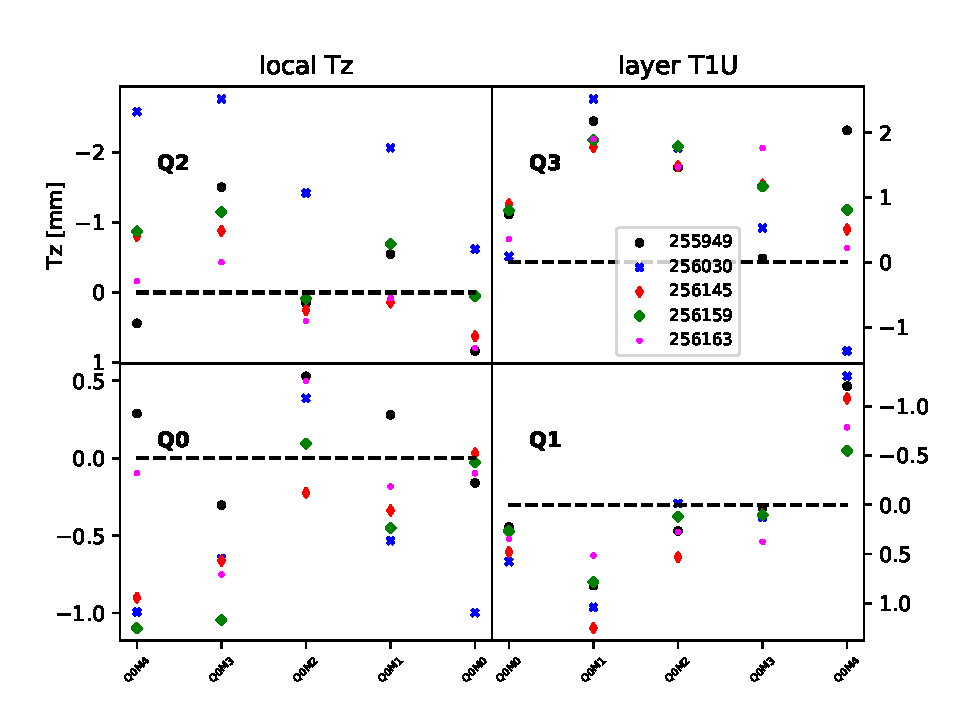
\includegraphics[width=0.9\textwidth]{plots/stability_plots/diff_MD_T1U_Tz.pdf}
%         \end{figure}
%       \end{column}
%   \end{columns}
% \end{frame}

\end{document}
